\section{Extending Electron Coherence}

\subsection{Spin-Echo}
In a spin-echo experiment a Ramsey experiment is performed with a small difference. An additional $\pi$ pulse is applied in the middle of the experiment exactly between the $\pi/2$ pulses. This pulse effectively turns the nuclear-spin environment upside-down halfway trough the experiment, making the qausi-static-part of the dephasing during the first and the second part of the free evolution cancel each other out, substantially increasing coherence on short-timescales ($\tau \ll T_2 $)
\footnote{ $T_2$ is a measure for decoherence. It is similar to $T_2^*$ but does not include variations between experiments. $T_2$ is defined as the $1/e$ time of the decay of a spin-echo experiment.}.
On longer timescales the difference between the initial part of the evolution and the final part of the evolution becomes larger making the initial and final part no longer cancel each other out.
\subsection{Dynamical Decoupling}
A natural way of extending the short timescale behavior of the spin-echo to longer timescales is by applying more $\pi$-pulses. This procedure known as dynamical-decoupling can dramatically improve coherence times by decoupling the central-spin from the environment\citep{Lange2010Universal}.

Although dynamical-decoupling improves the coherence of the central spin by decoupling from the environment, the central spin is also decoupled from other spins preventing direct two-qubit gates. It was demonstrated by \citet{Sar2012DecoherenceProtected} how to incorporate dynamical decoupling in a universal gate design by implementing Grover's algorithm.
Using this technique \citet{Taminiau2012Detection} used the extended coherence to detect and control weakly-coupled carbon spins, before implementing three-qubit quantum-error-correction (QEC) \citep{Taminiau2014Universal}.

As these experiments where performed with NV-centers at Room temperature they lack the option to do single-shot readout required to act on a measurement outcome\footnote{@Tim, I think this can be worded more concisely. Do you have any ideas?}. An essential feature for the parity measurements that form the basis of measurement-based QEC and surface codes.

\subsection{Dynamical decoupling spectroscopy}
As we cannot perform an ESR experiment while decoupling a different technique must be used to resolve and address additional spins.
In order to resolve additional spins we perform a dynamical decoupling spectroscopy, resulting in a fingerprint of the nuclear-spin environment\citep{Taminiau2012Detection}.

In a dynamical decoupling spectroscopy experiment the electron is prepared in the $|X\rangle = |0\rangle +|1\rangle$ state. It is subjected to a decoupling sequence consisting of N/2 blocks of the form {$\tau - \pi -2\tau-\pi-\tau$}, and concluded by measuring $\langle X\rangle $. The fingerprint is the result of many repetitions for a range of inter-pulse delays $2\tau$. $\pi$ is a $\pi$-pulse.

Part of a dynamical decoupling spectroscopy can be seen in \cref{fig:FP}. The spectroscopy was performed for N = 8, 16, 32 and 64 pulses. For N = 8, 16 and 32 pulses this was done between $\tau = 2 \mu \mathrm{s}$  and $72 \mu \mathrm{s}$ and for N = 64 this was done up to $\tau = 52 \mu \mathrm{s}$. A reference to the full spectroscopy can be found in \cref{chap:Fingerprint_data_appendix}.

\begin{figure}[htbp]

    \begin{subfigure}[t]{\textwidth}\centering
        \caption{}
        \begin{tikzpicture}
            \node[anchor=south west,inner sep=0] at (0,0) {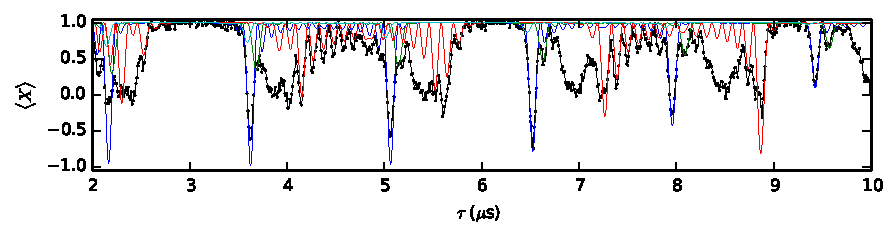
\includegraphics{Img/fingerprint16.pdf}};
            \node[font=\small, text = blue] at (4.05,1.7)  {1};
            \node[font=\small, text = green] at (9.3,2.9) {2};
            \node[font=\small, text = red] at (5.3,2.5) {3};
            \node[font=\small, text = cyan] at (4.0,3.35) {4};
            % \draw[help lines,xstep=1,ystep=1] (0,0) grid (10,3);
            % \foreach \x in {1,2,...,10} { \node [anchor=north] at (\x,0) {\x}; }
            % \foreach \y in {1,2,...,3} { \node [anchor=east] at (0,\y) {\y}; }
        \end{tikzpicture}
        \label{fig:FP16}
    \end{subfigure}

    \begin{subfigure}[t]{\textwidth}\centering

    \caption{}
    \begin{tikzpicture}
        \node[anchor=south west,inner sep=0] at (0,0) {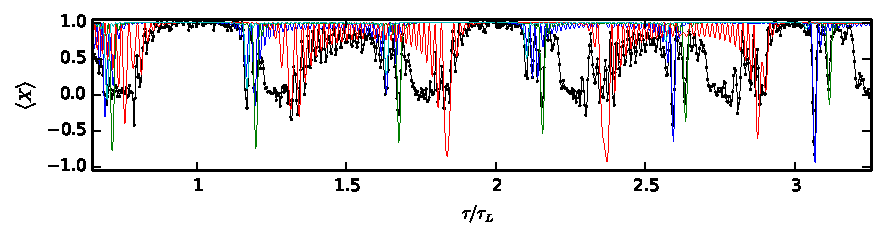
\includegraphics{Img/fingerprint32.pdf}};
        \node[font=\small, text = blue] at (11.2,1.9) {1};
        \node[font=\small, text = blue] at (4.0,2.8)  {1};
        \node[font=\small, text = green] at (6.6,1.8) {2};
        \node[font=\small, text = red] at (7.4,1.8) {3};
        \node[font=\small, text = cyan] at (4.05,2.5) {4};
        % \draw[help lines,xstep=1,ystep=1] (0,0) grid (10,3);
        % \foreach \x in {1,2,...,10} { \node [anchor=north] at (\x,0) {\x}; }
        % \foreach \y in {1,2,...,3} { \node [anchor=east] at (0,\y) {\y}; }
    \end{tikzpicture}
    \label{fig:FP32}
    \end{subfigure}
    \caption{Part of a fingerprint resulting from a dynamical-decoupling-spectroscopy experiment performed at 304G. A reference to the full spectroscopy can be found in \cref{chap:Fingerprint_data_appendix}.  Colored lines represent computed responses of carbon spins. Responses were calculated using \cref{eq:contrast_single_carbon_spin} with hyperfine parameters from \cref{tbl:HF_par}. }
    \label{fig:FP}
\end{figure}
